\documentclass[11pt]{article}

% ── Packages ────────────────────────────────────────────────
\usepackage[margin=1in]{geometry}
\usepackage{amsmath, amssymb, amsthm}
\usepackage{booktabs}
\usepackage{graphicx}
\usepackage{hyperref}
\usepackage{natbib}
\usepackage{setspace}
\usepackage{microtype}
\usepackage{enumitem}
\usepackage{caption}
\usepackage{subcaption}
\usepackage{xcolor}
\usepackage{float}
% code packages
\usepackage{listings}
\usepackage{inconsolata}
\lstset{basicstyle=\ttfamily\footnotesize,breaklines=true}
\usepackage{csvsimple}
\usepackage{booktabs}

% ── Hyperref setup ──────────────────────────────────────────
\hypersetup{
    colorlinks = true,
    linkcolor  = black,
    citecolor  = black,
    urlcolor   = blue
}

% ── Theorem environments ────────────────────────────────────
\newtheorem{theorem}{Theorem}
\newtheorem{proposition}{Proposition}
\newtheorem{lemma}{Lemma}
\newtheorem{corollary}{Corollary}
\theoremstyle{definition}
\newtheorem{definition}{Definition}
\newtheorem{assumption}{Assumption}
\theoremstyle{remark}
\newtheorem{remark}{Remark}

% ── Spacing ─────────────────────────────────────────────────
\onehalfspacing

% ── Title block ─────────────────────────────────────────────
\title{Love of Variety Model and Simulation}
\author{Tate Mason}
\date{\today}

% ============================================================
\begin{document}
\maketitle
\thispagestyle{empty}

% ── Abstract ────────────────────────────────────────────────

\newpage
\setcounter{page}{1}

\section{Motivation}

In canonical IO models, love of variety is not explicitly considered as a part of utility. Instead, it is baked into other parameters, potentially biasing the true value attributed to quality, whether observed or unobserved. In this paper, I attempt to explicitly model love of variety as a part of the consumer's utility. Further, I will show how firms can infer a consumer's value for varied products in advertising to lure them towards certain products or product spaces.

I contribute to three main strands of literature: love of variety and habit formation, dynamic advertising, and dynamic discrete choice estimation. For love of variety, I am adding a new way of thinking about how this preference is measured, merging some habit stock methods with preference for distance from habit. For advertising, I am bringing the love-of-variety context as a way for firms to learn about consumers and more effectively advertise to consumers depending on LOV type. Finally, for dynamic discrete choice, I am hoping to implement neural network estimation, allowing me to make computational efficiency gains of traditional SMM or MLE methods.

The rest of the document is structured as follows: section II describes the consumers' problem, section III goes into the simulation process, and section IV describes my next steps.

\section{Model}

\subsection{Consumer's Problem}
The consumer's problem is to maximize utility subject to their choice set. The utility function is as follows:

\begin{equation}
  U_{ijt} = \beta_i X_{jt} + \gamma_{i}(\Sigma_{ijt})^2 + \kappa a_{jt} - \alpha p_{jt} + \xi_j + \epsilon_{ijt}
\end{equation}

\begin{gather*}
  \Sigma_{ijt} = X_{jt}-\bar{X}_{it}
\end{gather*}

Here, $U_{ijt}$ is the utility of consumer $i$ who chooses product $j$ in period $t$. Utility depends on utility from characteristics associated with product $X_jt$, $\beta_i$,
love of variety $\gamma_i$, how different your current choice is from the mean $\Sigma_{ijt}$, advertising $a_{jt}$, prices $p_{jt}$, and unobserved quality $\xi_j$.
Further, a gumbel shock $\varepsilon_{ijt}$ also impacts utility. This is what allows us to construct choice probabilities as follows:

\begin{equation}
  P_{ijt} = \frac{e^{U_{ijt}}}{1 + \sum_{k} e^{U_{ikt}}}
\end{equation}

\section{Simulation}

To understand model behavior, I first do Monte Carlo exercises across different environments. This will be replaced by Nielsen scanner data once access is gained.

\subsection{Parameters}

\begin{table}[hbtp]
  \centering
  \begin{tabular}{lcl}
    \toprule
    Parameter & Value & Description \\
    \midrule
    $\beta_i$ & \{1, 2.5, 4\} & Consumer preference for product attributes \\
    $\gamma_i$ & \{1, 2.5, 4\} & Consumer love of variety \\
    $\kappa$ & 3 & Advertising cost parameter \\
    $\alpha_j$ & 0 & Price sensitivity \\
    $\xi_j$ & 0 & Unobserved quality \\
    \bottomrule
  \end{tabular}
  \caption{Simulation Parameters}
  \label{tab:model_parameters}
\end{table}

Still working on parameter scaling, subject to change.

\subsection{Simulation Procedure}

I have simulated two specifications so far: one in which the mean is fixed as the mean of an ordinal product set and one with a mean informed by individual histories over products from a normal distribution. Below I go into each of these with graphs of choice probabilities in a market with one consumer.

\subsection{Set Mean}
In the first simulation routine, The product set $J$ is defined as $J = \{1.0, 2.0, 3.0, 4.0, 5.0\}$. Consider this the most simple form available, where $\bar{X}_it = 2.5$, the mean of $J$. Thus, $\Sigma_{ijt} = X_{jt} - 2.5$. Therefore, the only thing changing over time is the new epsilon draw each period. This specification also sets $a_{jt}=0$ to really allow the $\beta_i, \ \gamma_i$ regimes to show their behavior.

\begin{figure}[H]
  \centering
    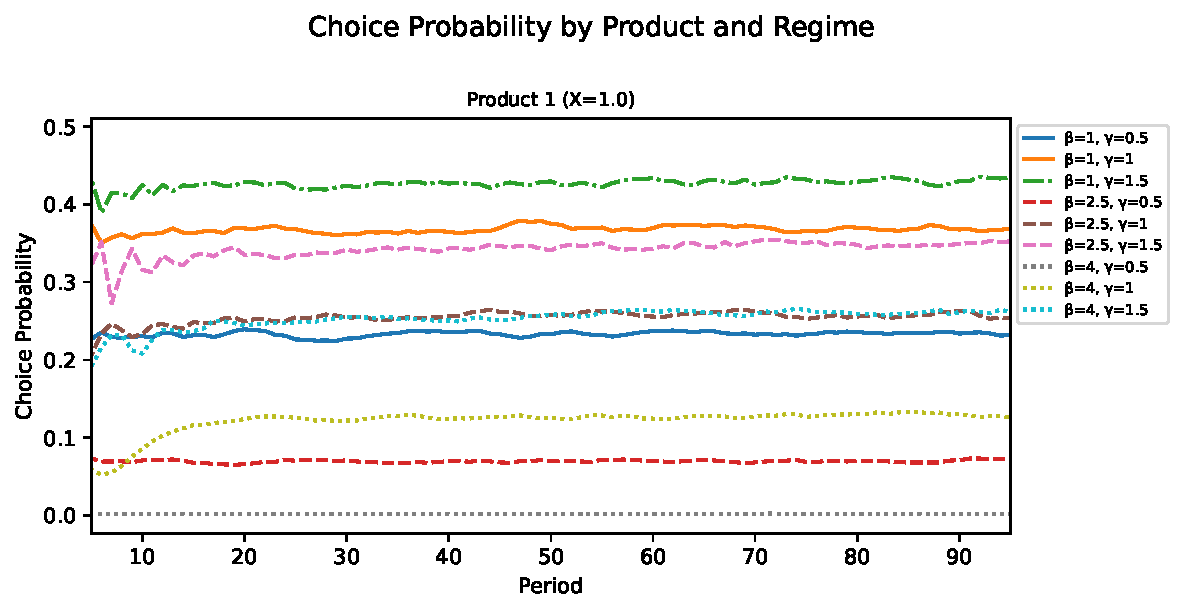
\includegraphics[width=\textwidth]{../../Output/fixed_mean_choice_prob_product_1.pdf}
    \caption{Choice Probability of Product 1 by Regime}
    \label{fig:choice_prob_product_1}
\end{figure}

\begin{figure}[H]
  \centering
    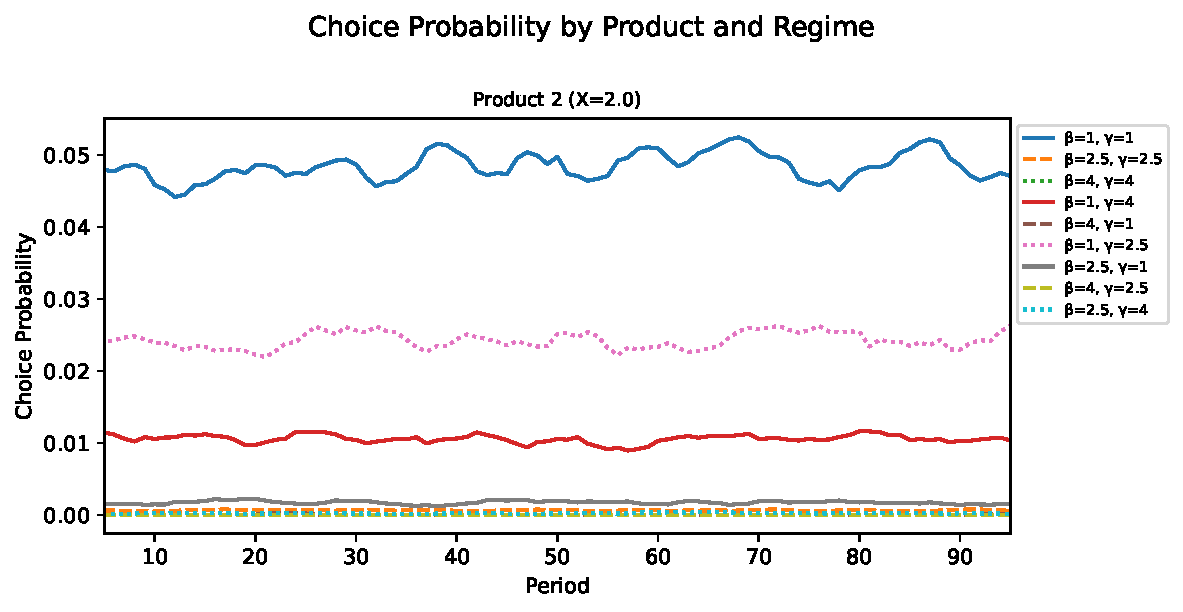
\includegraphics[width=\textwidth]{../../Output/fixed_mean_choice_prob_product_2.pdf}
    \caption{Choice Probability of Product 2 by Regime}
    \label{fig:choice_prob_product_2}
\end{figure}

\begin{figure}[H]
  \centering
    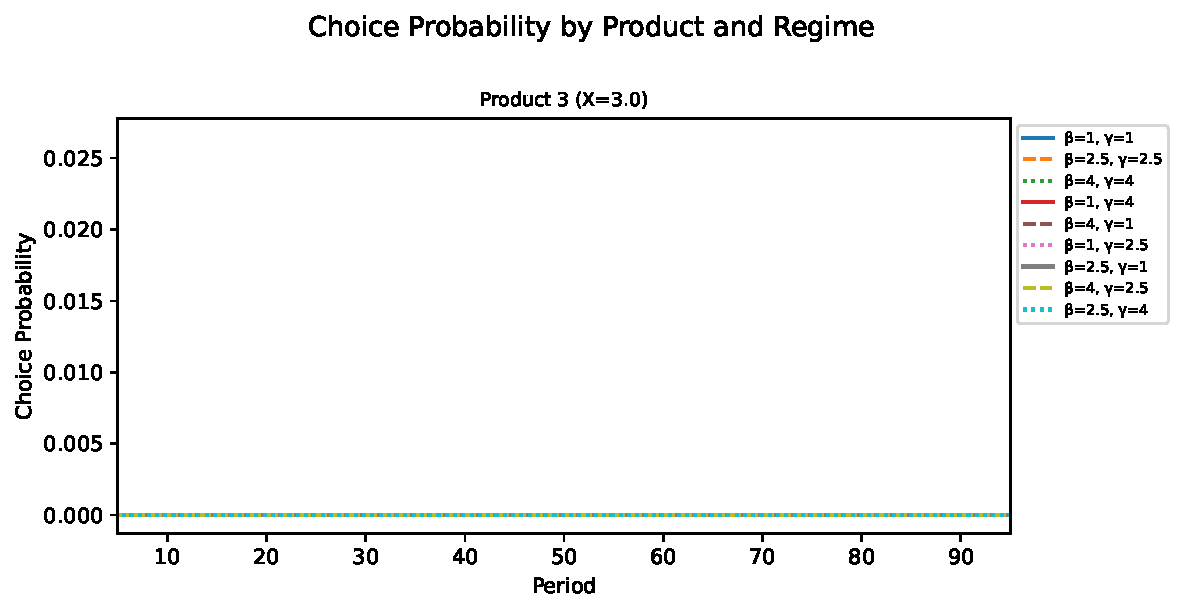
\includegraphics[width=\textwidth]{../../Output/fixed_mean_choice_prob_product_3.pdf}
    \caption{Choice Probability of Product 3 by Regime}
    \label{fig:choice_prob_product_3}
\end{figure}

\begin{figure}[H]
    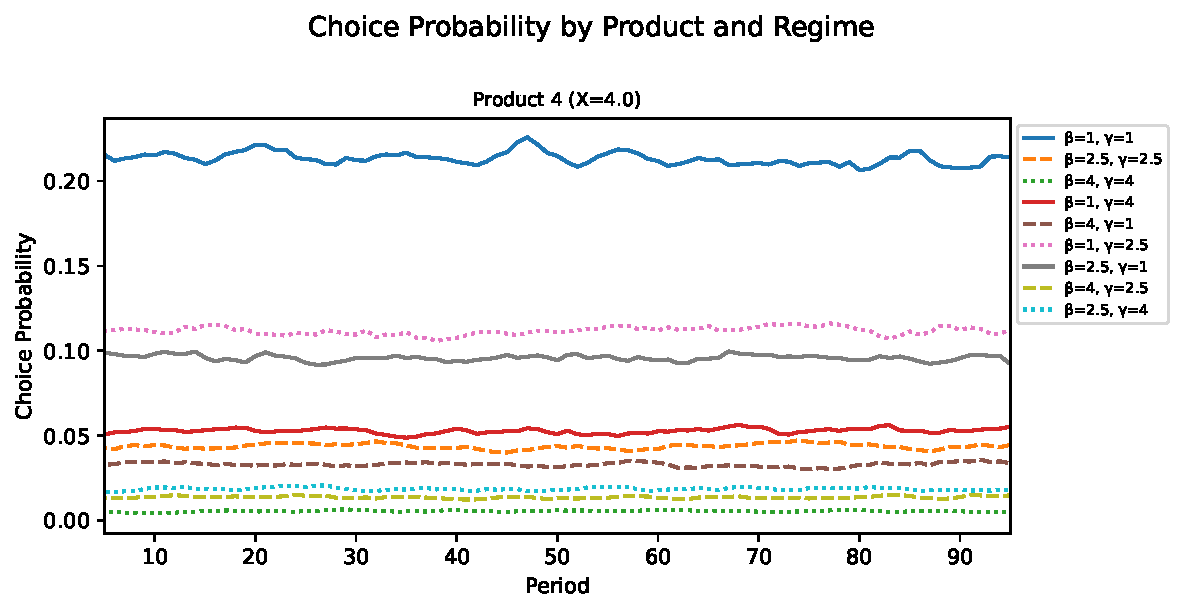
\includegraphics[width=\textwidth]{../../Output/fixed_mean_choice_prob_product_4.pdf}
    \caption{Choice Probability of Product 4 by Regime}
    \label{fig:choice_prob_product_4}
\end{figure}

\begin{figure}[H]
  \centering
    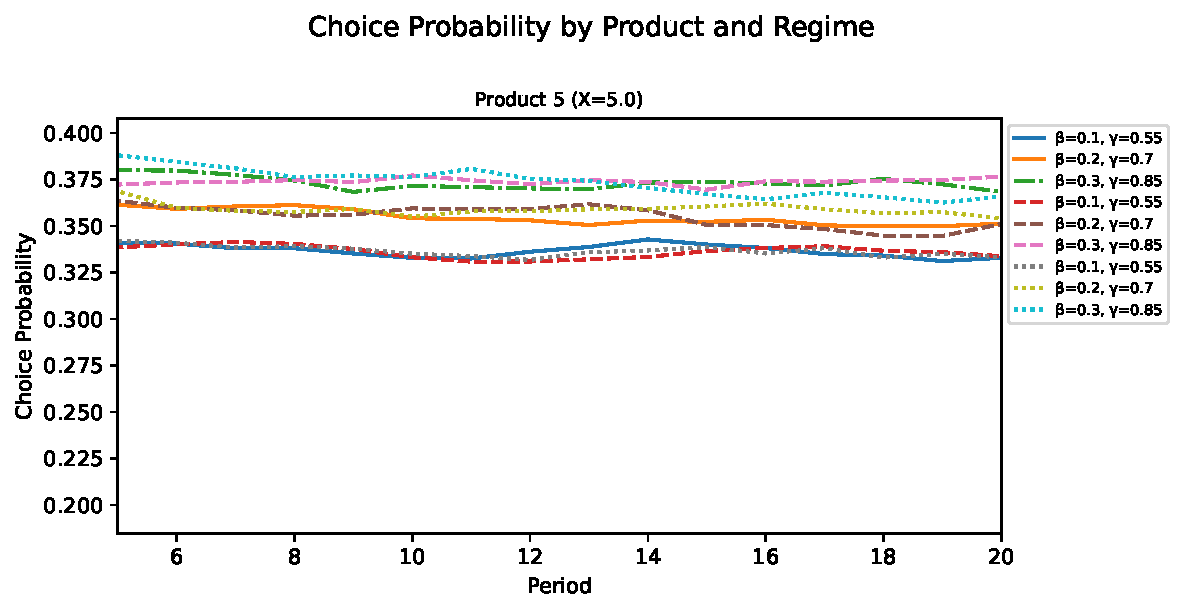
\includegraphics[width=\textwidth]{../../Output/fixed_mean_choice_prob_product_5.pdf}
    \caption{Choice Probability of Product 5 by Regime (Fixed Advertising $a=0.2$)}
    \label{fig:choice_prob_product_5}
\end{figure}


\subsection{Prior Mean}

In this routine, I implemented an idea Josh had in a meeting: the consumer has a history of products they like. So, to implement a version of this, I sim five periods before my main simulation of 100 periods to create a mean over $X$'s as they enter the model. All else is the same as above.

\clearpage

\begin{figure}[H]
  \centering
  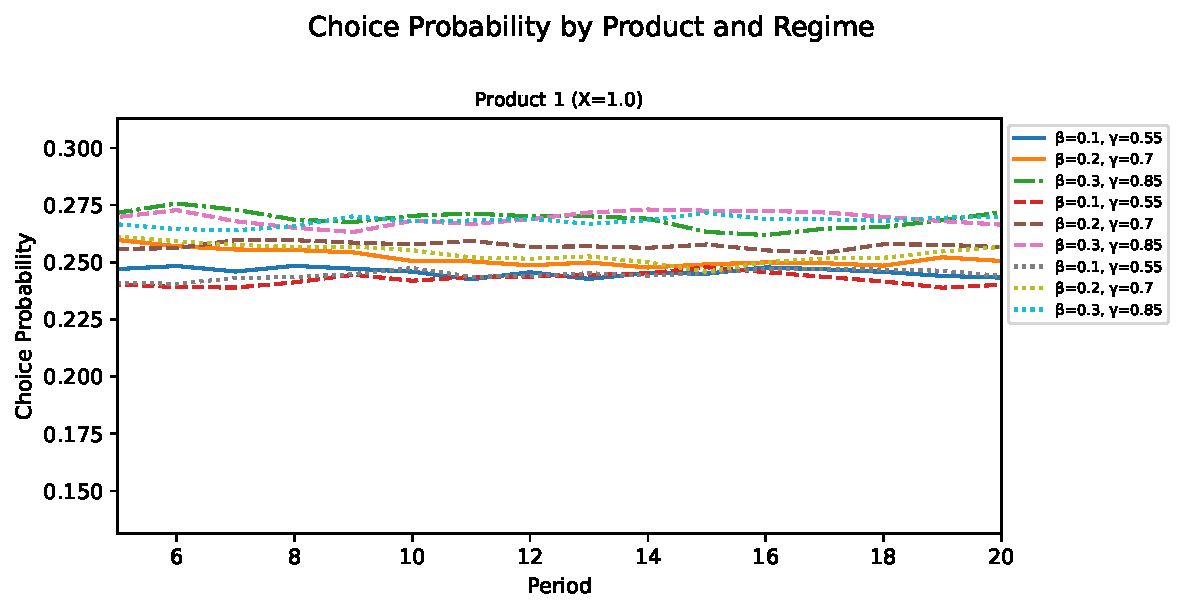
\includegraphics[width=0.7\textwidth]{../../Code/prior_mean_choice_prob_product_1.pdf}
  \caption{Choice Probability of Product 1 by Regime (Fixed Advertising $a=2$)}
  \label{fig:choice_prob_product_1}
\end{figure}

\begin{figure}[H]
  \centering
  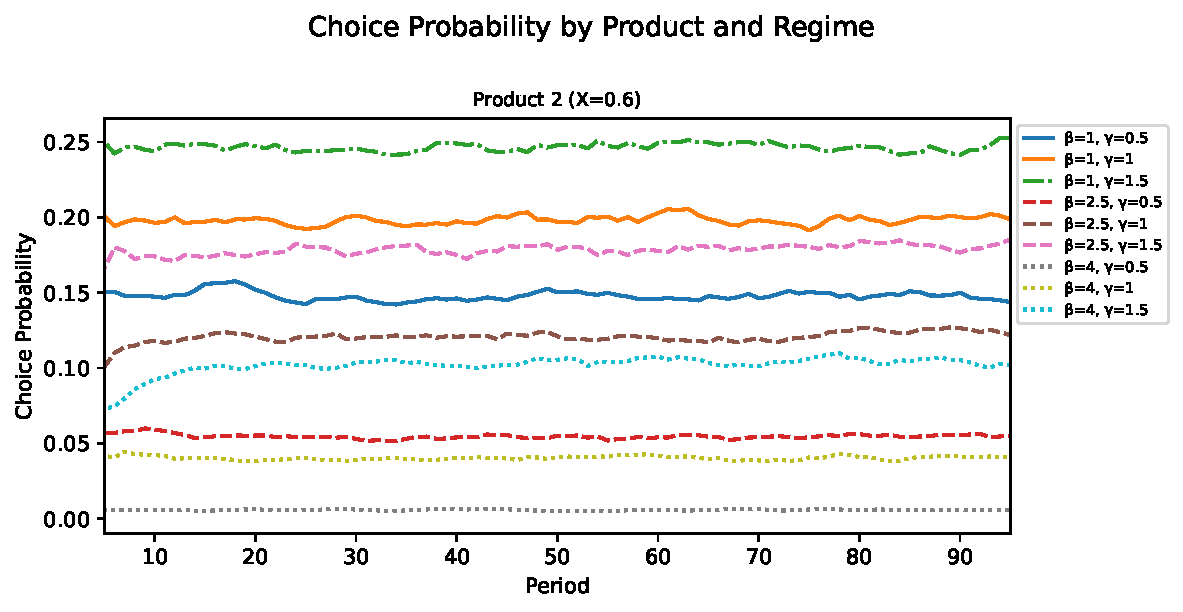
\includegraphics[width=0.7\textwidth]{../../Code/prior_mean_choice_prob_product_2.pdf}
  \caption{Choice Probability of Product 2 by Regime (Fixed Advertising $a=2$)}
  \label{fig:choice_prob_product_2}
\end{figure}

\begin{figure}[H]
  \centering
  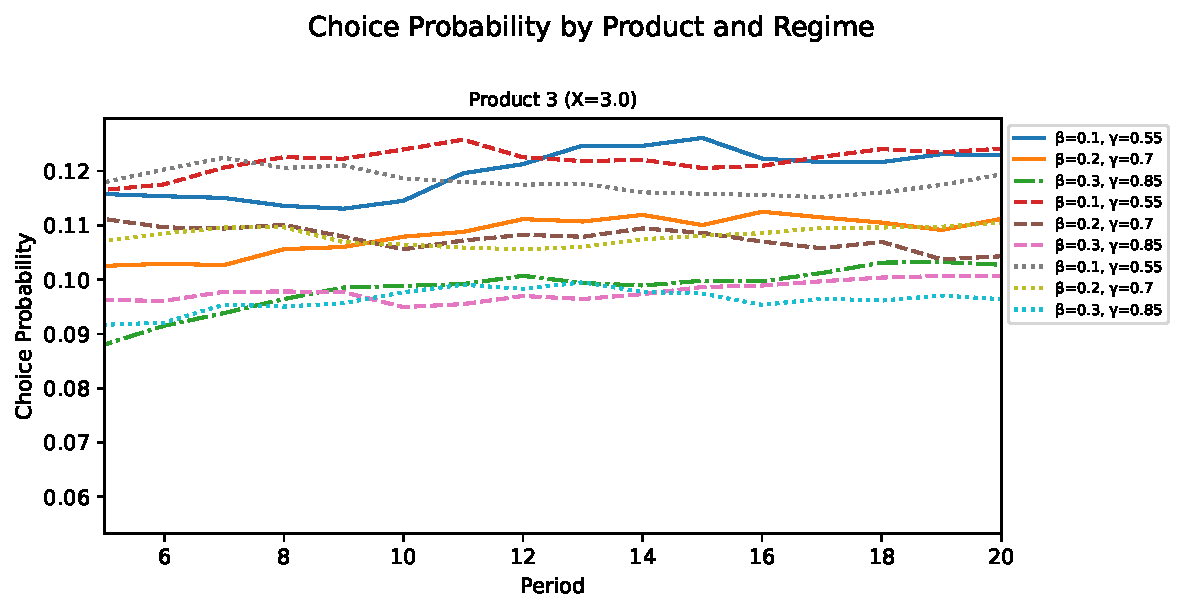
\includegraphics[width=0.7\textwidth]{../../Code/prior_mean_choice_prob_product_3.pdf}
  \caption{Choice Probability of Product 3 by Regime (Fixed Advertising $a=2$)}
  \label{fig:choice_prob_product_3}
\end{figure}

\begin{figure}[H]
  \centering
  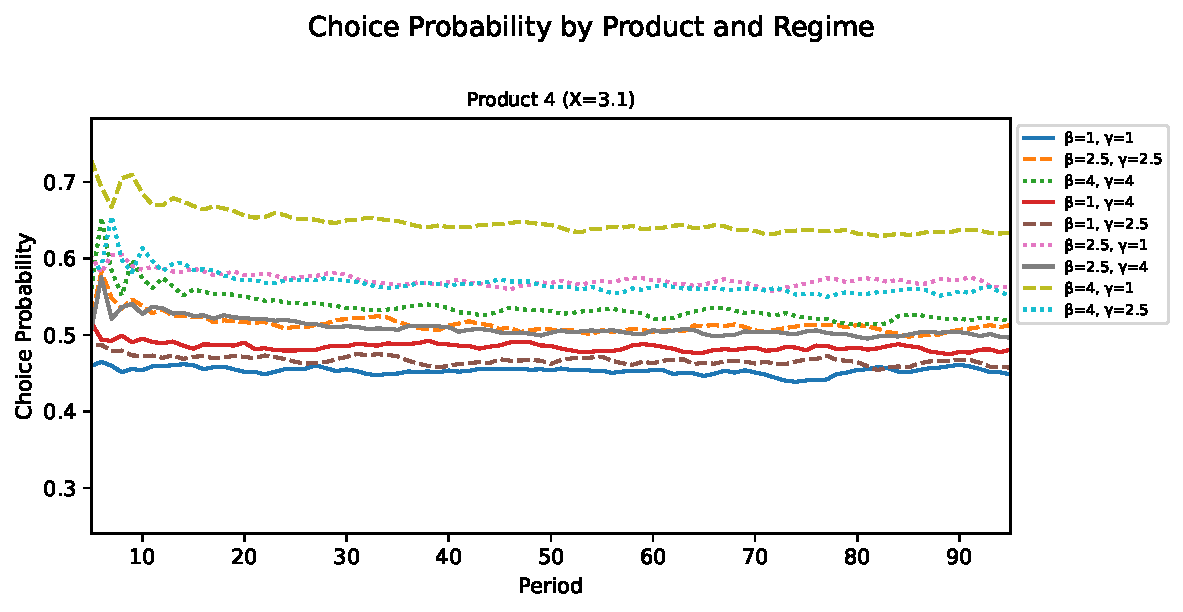
\includegraphics[width=0.7\textwidth]{../../Code/prior_mean_choice_prob_product_4.pdf}
  \caption{Choice Probability of Product 4 by Regime (Fixed Advertising $a=2$)}
  \label{fig:choice_prob_product_4}
\end{figure}

\begin{figure}[H]
  \centering
  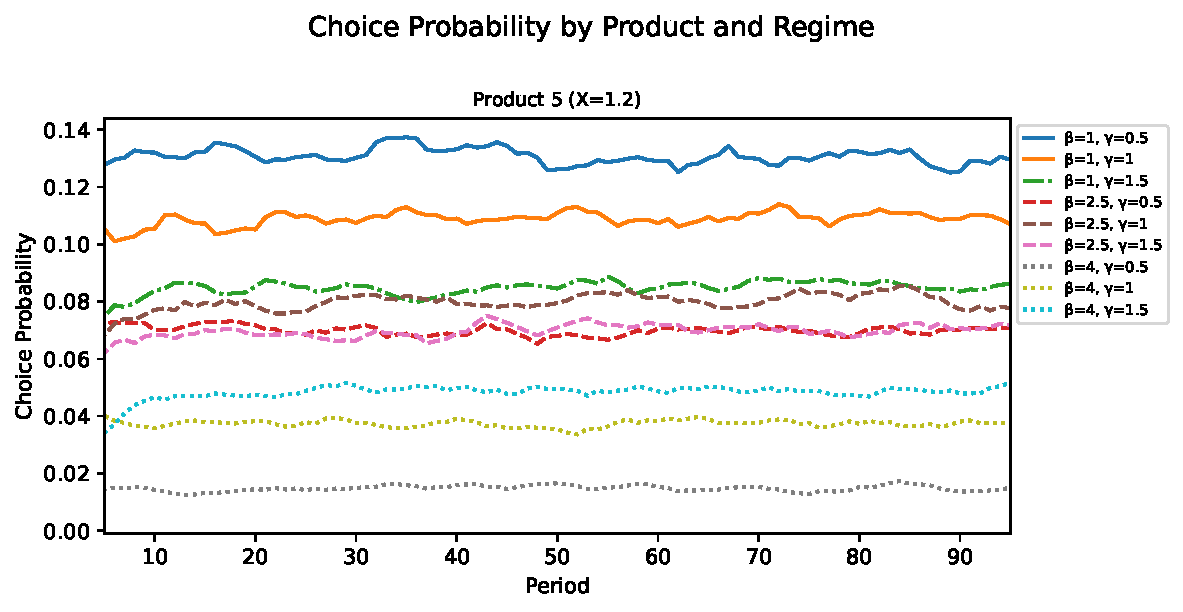
\includegraphics[width=0.7\textwidth]{../../Code/prior_mean_choice_prob_product_5.pdf}
  \caption{Choice Probability of Product 5 by Regime (Fixed Advertising $a=2$)}
  \label{fig:choice_prob_product_5}
\end{figure}

This specification yields interesting patterns. Particularly, the regime $(\beta=1, \gamma=2.5)$. This regime will flip between products, choosing all but product 4. This is because the utility gain is outweighed enough by the penalty to encourage variety. In the other specification, the same regime choosed product 3 70\% of the time. 
So having a dynamic mean informed by priors seems to encourage the behaviors sought after. The regime $(\beta=4, \gamma=1)$ picks the highest value product 100\% of the time. $(\beta=4, \gamma=2.5)$ converges to product 4 100\% of the time after about 30 periods, showing that the penalty does have an effect early, but the utility gain is enough to eventually win out into steady state.

\section{Next Steps}

Next, I would like to go to 5 consumers, and see how things change. I also want to see how pulling from $\gamma\sim N(0, \sigma_{\gamma})$ affects things. Of course, I also need to start really thinking about the firm side and the consumer's value function. I am also working on beginning my literature review, which has inspired some interesting ideas.

\end{document}
